\chapter{Zbiór danych i metodyka badań}

Specyfika problemu rozpoznawania trzymanych obiektów trójwymiarowych wymaga przygotowania własnego zbioru danych. Niniejszy rozdział opisuje proces pozyskiwania danych, ich oznaczania, przyjęty sposób podziału na zbiory oraz sposób, w jaki przeprowadzono eksperymenty.

\section{Zbiór danych}

Stworzenie odpowiedniego zbioru danych jest kluczowe dla przeprowadzenia eksperymentów i oceny jakości detekcji. Kluczowe jest, aby odpowiadał on rzeczywistym zastosowaniom systemu, a także aby był wystarczająco zróżnicowany i reprezentatywny dla problemu.

\subsection{Charakterystyka zbioru danych}

Przygotowany zbiór danych składa się z 4666 obrazów JPEG o rozdzielczości $1920\times1440$ podzielonych na zbiory treningowy, walidacyjny i testowy. Przedstawiają one osobę siedzącą przed kamerą, manipulującą w dłoniach bryłami należącymi do jednej z 6 klas obiektów:
\begin{itemize}
    \item sześcian,
    \item prostopadłościan,
    \item kula,
    \item walec,
    \item stożek,
    \item czworościan.
\end{itemize}
Obrazy w zbiorze zostały pozyskane z nagrań wideo, z zachowaniem występowania wszystkich klas w każdym nagraniu.

Liczbę obrazów w poszczególnych zbiorach z podziałem na klasy i tła przedstawiono w tabeli~\ref{tab:dataset_split}. Podział danych został wykonany w taki sposób, aby dane z jednego nagrania nie znalazły się w kilku zbiorach. Ogranicza to ryzyko przecieku danych oraz możliwość zawyżenia wyników poprzez rozpoznanie obiektu bazując jedynie na wyglądzie sceny, a nie na faktycznym kształcie bryły.

Pełen zbiór danych wraz z adnotacjami zawiera 4666 obrazów i 4666 odpowiadających im plików adnotacji w formacie YOLO, a także 4 pliki tekstowe. Łączny rozmiar zbioru danych to $3,19$ GB.

\begin{table}
    \centering
    \caption{Podział zbioru danych na zbiory treningowy, walidacyjny i testowy.}
    \label{tab:dataset_split}
    \begin{tabularx}{\textwidth}{l|XXX}
        \toprule
        \textbf{Klasa}            & \textbf{Zbiór treningowy} & \textbf{Zbiór walidacyjny} & \textbf{Zbiór testowy} \\
        \midrule
        \textbf{Sześcian}         & 493                       & 54                         & 90                     \\
        \textbf{Kula}             & 334                       & 30                         & 51                     \\
        \textbf{Walec}            & 377                       & 54                         & 68                     \\
        \textbf{Prostopadłościan} & 563                       & 47                         & 86                     \\
        \textbf{Czworościan}      & 923                       & 85                         & 18                     \\
        \textbf{Stożek}           & 424                       & 48                         & 52                     \\
        \textbf{Tło}              & 668                       & 89                         & 112                    \\
        % \addlinespace
        \midrule

        \textbf{Razem}            & 3782                      & 407                        & 477                    \\
        \bottomrule
    \end{tabularx}
\end{table}

Dodatkowa charakterystyka zbioru uczącego została przedstawiona na rysunku~\ref{fig:dataset_labels}. Oprócz liczności poszczególnych klas przedstawiono na nim również rozkład położenia ramek ograniczających oraz ich znormalizowane wymiary. Większość z nich znajduje się w centralnej części obrazu, co jest skutkiem przyjętego sposobu rejestrowania materiałów wideo.

\begin{figure}[h]
    \centering
    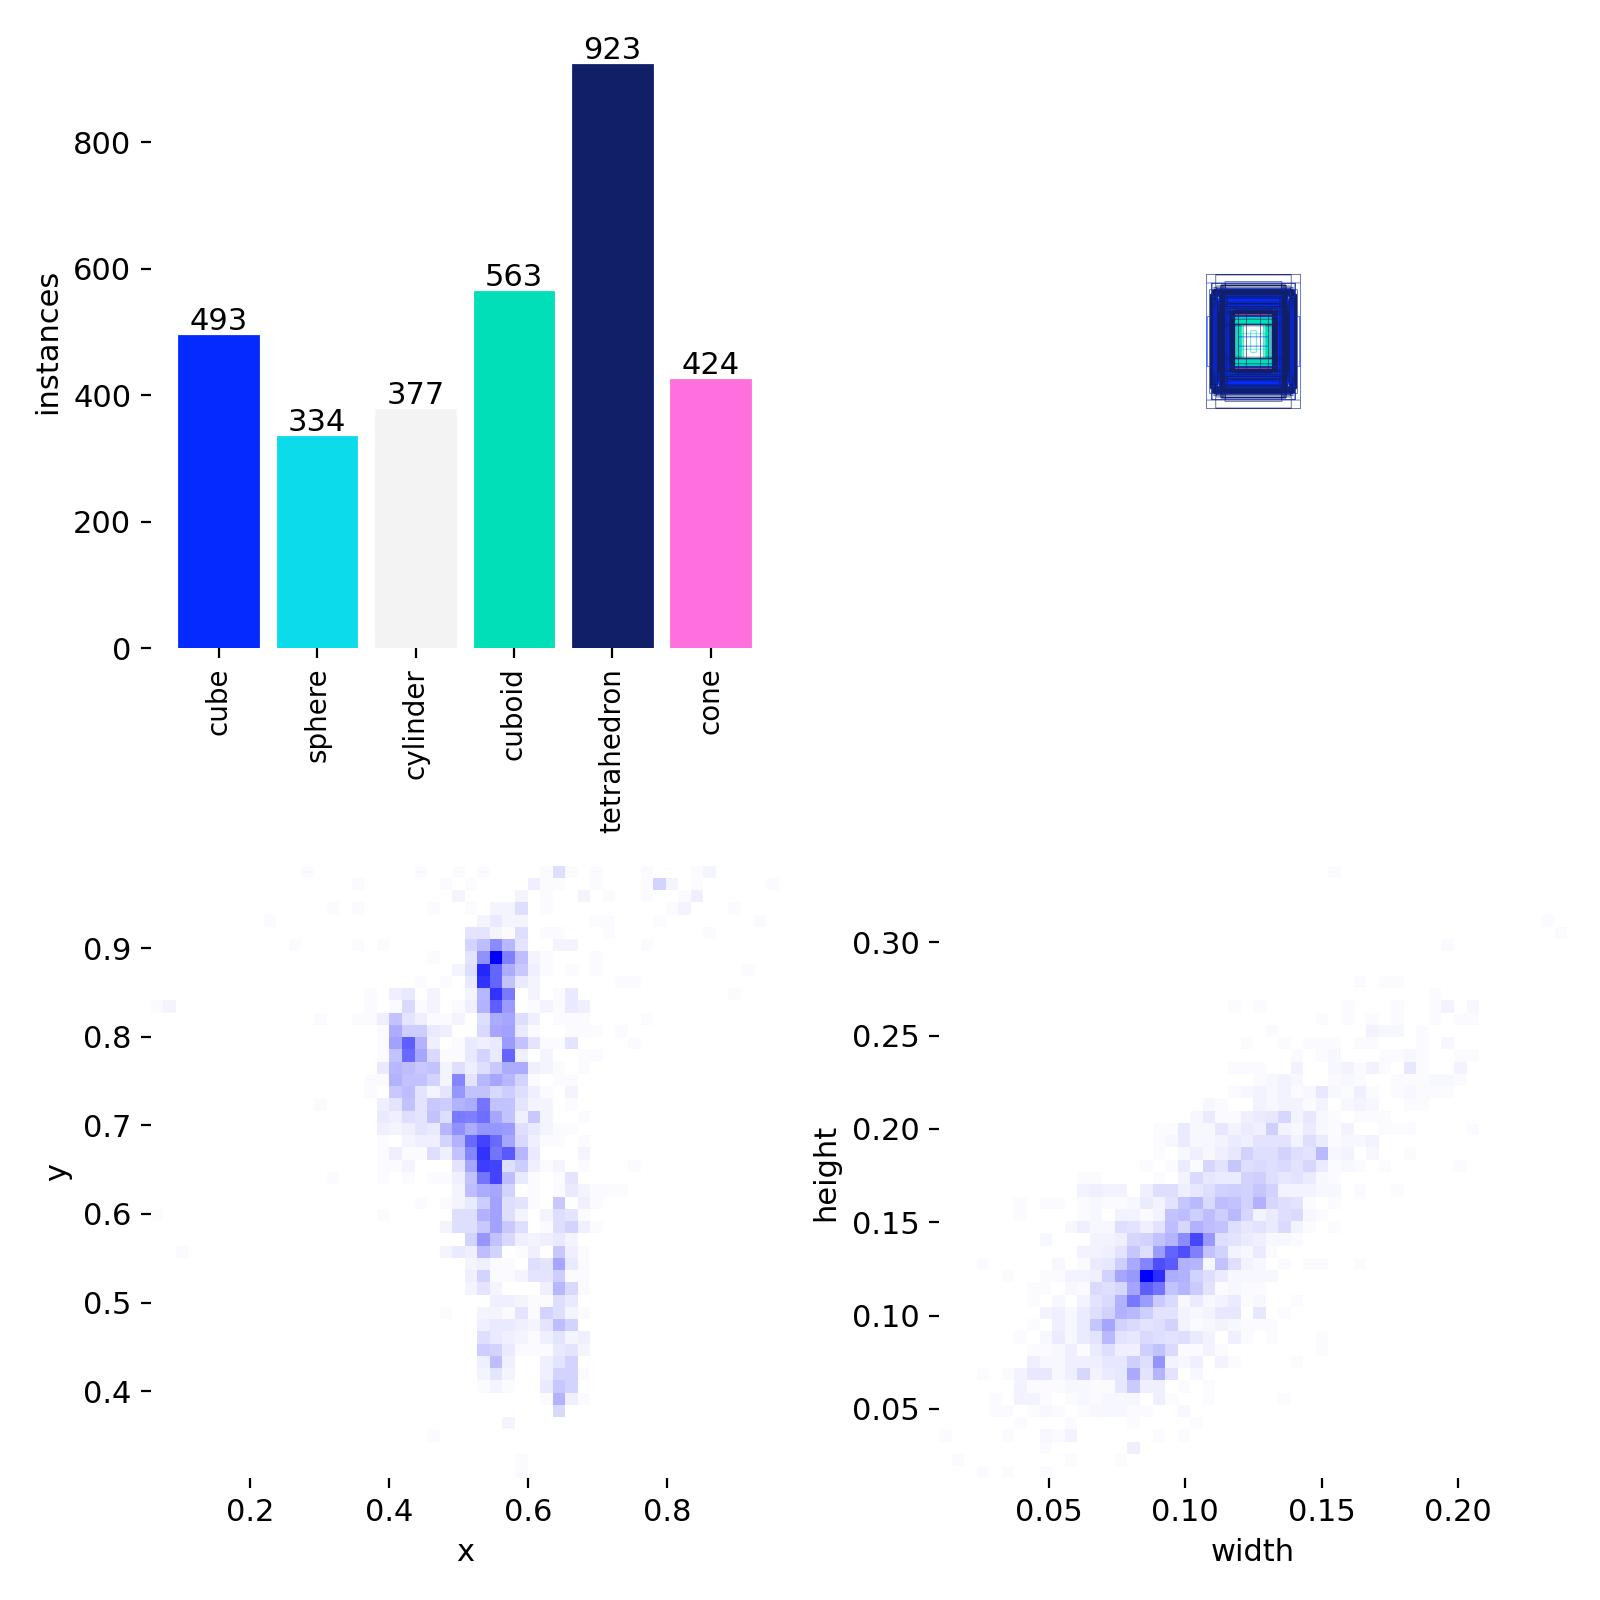
\includegraphics[width=0.8\textwidth]{./graf/labels.jpg}
    \caption{Rozkład klas oraz położenia ramek ograniczających w zbiorze treningowym.}
    \label{fig:dataset_labels}
\end{figure}

\subsection{Proces pozyskiwania i oznaczania danych}

Pierwszym etapem przygotowania zbioru danych było nagranie materiałów wideo zawierających wspomniane wcześniej widoki osoby manipulującej bryłami. Zarejestrowano je przy pomocy nieruchomego urządzenia mobilnego Samsung Galaxy S25 w rozdzielczości $1920\times1440$ i 30 klatkach na sekundę. Zostały one zrealizowane w różnych warunkach oświetleniowych z wykorzystaniem światła dziennego i sztucznego, z różnymi osobami i w różnych ubraniach. Na każdym nagraniu osoba manipuluje każdą z przygotowanych brył sposób odpowiadający przewidywanemu scenariuszowi użycia systemu. Ostatecznie nagrano 9 filmów o łącznej długości 14 minut i 16 sekund. Następnie, korzystając z przygotowanego skryptu (por.~\ref{ssec:extractor}), z wszystkich nagrań wyekstrahowano 4666 obrazów w formacie JPEG.

W następnym kroku obrazy należało oznaczyć, czyli przygotować adnotacje obiektów, które się na nich znajdują. Do tego zadania wykorzystano narzędzie \texttt{CVAT} \cite{bib:cvat} rozwijane przez firmę cvat.ai corporation. Zostało ono wybrane ze względu na możliwość pracy w przeglądarce internetowej, a także półautomatyczne oznaczanie obiektów korzystając z wcześniej wytrenowanego modelu detekcji. Niestety, w trakcie oznaczania napotkano problemy z uruchomieniem modelu w narzędziu, co skutkowało koniecznością ręcznego oznaczania wszystkich obiektów i rezygnacji z rozszerzenia zbioru o dodatkowe obrazy. Podczas pracy z narzędziem korzystano również z serwisu Amazon S3 do przechowywania danych w chmurze. Dzięki niemu nie zaistniała konieczność przesyłania dużych ilości danych pomiędzy wykorzystywanymi platformami.

\subsection{Podział danych na zbiory treningowy, walidacyjny i testowy}

Po oznaczeniu danych należało je podzielić na zbiory treningowy, walidacyjny i testowy. Wykonano ręczny podział danych tak, aby obrazy z pojedynczego nagrania nie były rozdzielone pomiędzy różne zbiory. Zadbano równocześnie, aby zbiór treningowy zawierał zróżnicowane obrazy, a zbiory walidacyjny i testowy zawierały wszystkie klasy oraz możliwie zróżnicowane przykłady scen. Nagrania, z których obrazy znalazły się w zbiorach treningowym i walidacyjnym zostały zarejestrowane pojedynczego dnia, a nagrania dla zbioru testowego zostały zarejestrowane kilka dni później. Ostateczny udział obrazów w pełnym zbiorze danych wynosił $81\%$ dla zbioru treningowego, $8,7\%$ dla zbioru walidacyjnego i $10,2\%$ dla zbioru testowego. Zrezygnowano z wykorzystania skryptu \texttt{split\_dataset.py} do podziału danych, aby nie mieszać obrazów, a tym samym wykluczyć możliwość rozpoznania obiektów na podstawie wyglądu sceny. Szczegółowy udział filmów w poszczególnych zbiorach przedstawiono w tabeli~\ref{tab:video_split}.

\begin{table}[ht]
    \caption{Podział nagrań wideo pomiędzy zbiory treningowy, walidacyjny i testowy.}
    \label{tab:video_split}
    \begin{tabularx}{\textwidth}{X|llll}
        \toprule
        \textbf{Data nagrania} &
        \makecell[tl]{\textbf{Długość nagrania} \\mm:ss} &
        \makecell[tl]{\textbf{Liczba}           \\\textbf{obrazów}} &
        \textbf{Zbiór}         &
        \textbf{Udział}                         \\
        \midrule
        \makecell[tl]{13-05-2026                \\12:39} & 04:07 & 1481 & treningowy & \makecell[tl]{całościowy: $31,7\%$\\w zbiorze: $39,2\%$} \\
        \makecell[tl]{13-05-2026                \\12:45} & 02:21 & 843 & treningowy & \makecell[tl]{całościowy: $18,1\%$\\w zbiorze: $22,3\%$} \\
        \makecell[tl]{13-05-2026                \\12:50} & 01:37 & 581 & treningowy & \makecell[tl]{całościowy: $12,5\%$\\w zbiorze: $15,4\%$} \\
        \makecell[tl]{13-05-2026                \\12:53} & 01:22 & 493 & treningowy & \makecell[tl]{całościowy: $10,6\%$\\w zbiorze: $13,0\%$} \\
        \makecell[tl]{13-05-2026                \\12:58} & 01:04 & 384 & treningowy & \makecell[tl]{całościowy: $8,2\%$\\w zbiorze: $10,2\%$} \\
        \makecell[tl]{13-05-2026                \\13:02} & 01:08 & 407 & walidacyjny & \makecell[tl]{całościowy: $8,7\%$\\w zbiorze: $100\%$} \\
        \makecell[tl]{19-05-2026                \\14:03} & 0:54 & 164 & testowy & \makecell[tl]{całościowy: $3,5\%$\\w zbiorze: $34,4\%$} \\
        \makecell[tl]{19-05-2026                \\14:06} & 0:54 & 164 & testowy & \makecell[tl]{całościowy: $3,5\%$\\w zbiorze: $34,4\%$} \\
        \makecell[tl]{19-05-2026                \\14:10} & 0:49 & 149 & testowy & \makecell[tl]{całościowy: $3,2\%$\\w zbiorze: $31,2\%$} \\
        \bottomrule
    \end{tabularx}
\end{table}

Przeznaczenie poszczególnych zbiorów danych jest zgodne z przyjętymi w literaturze standardami oraz nie występuje nakładanie się ich zastosowań. Zbiór treningowy służy wyłącznie do trenowania modeli, zbiór walidacyjny do oceny jakości modeli w trakcie treningu, a zbiór testowy jest używany wyłącznie do oceny jakości modeli po zakończeniu treningu.

\subsection{Warianty danych wejściowych}

Podstawowym wariantem danych wejściowych jest obraz kolorowy w przestrzeni barw RGB. Stanowi on punkt odniesienia dla wszystkich eksperymentów.

Aby sprawdzić eksperymentalnie wpływ koloru na jakość detekcji, postanowiono przetestować zdolność modeli na danych wejściowych w dwóch wariantach: kolorowym (RGB) oraz w odcieniach szarości (grayscale). Konwersja na odcienie szarości została wykonana obliczając wartość ważonej luminancji z wykorzystaniem wzoru:
\begin{equation}
    Y = 0,299 \cdot R + 0,587 \cdot G + 0,114 \cdot B.
\end{equation}
Taki dobór wag najlepiej odzwierciedla wpływ poszczególnych kanałów na postrzeganą jasność obrazu przez ludzkie oko. Następnie wartość luminancji została powielona na wszystkie trzy kanały, aby zachować zgodność z oczekiwanym przez modele wejściem.

Zastosowanie w tym miejscu średniej wartości kolorów:
\begin{equation}
    Y = \frac{R + G + B}{3}
\end{equation}
nie zostało uznane za właściwe, ponieważ eksperyment ma na celu sprawdzenie, czy usunięcie informacji o barwie będzie miało wpływ na jakość detekcji, a średnia wartość kolorów nie odzwierciedla rzeczywistego wpływu poszczególnych kolorów na postrzeganą jasność obrazu.

Repozytorium z projektem zawiera również filtr Sobela, jednakże nie został on wykorzystany w eksperymentach ponieważ oczekujemy, że model będzie w stanie samodzielnie wyznaczyć krawędzie obiektów. Użycie klasycznego, deterministycznego operatora detekcji krawędzi skutkuje zatraceniem informacji o teksturze i rozkładzie jasności w obrębie obiektów. Ich utrata może skutkować obniżeniem jakości detekcji, szczególnie w przypadku obiektów, które nie mają wyraźnych krawędzi, np. kuli.

Porównanie obrazów w wariancie kolorowym z obrazami na których zastosowano opisane filtry przedstawiono na rysunku~\ref{fig:dataset_variants}.

\begin{figure}
    \centering
    \begin{subfigure}[b]{0.45\textwidth}
        \centering
        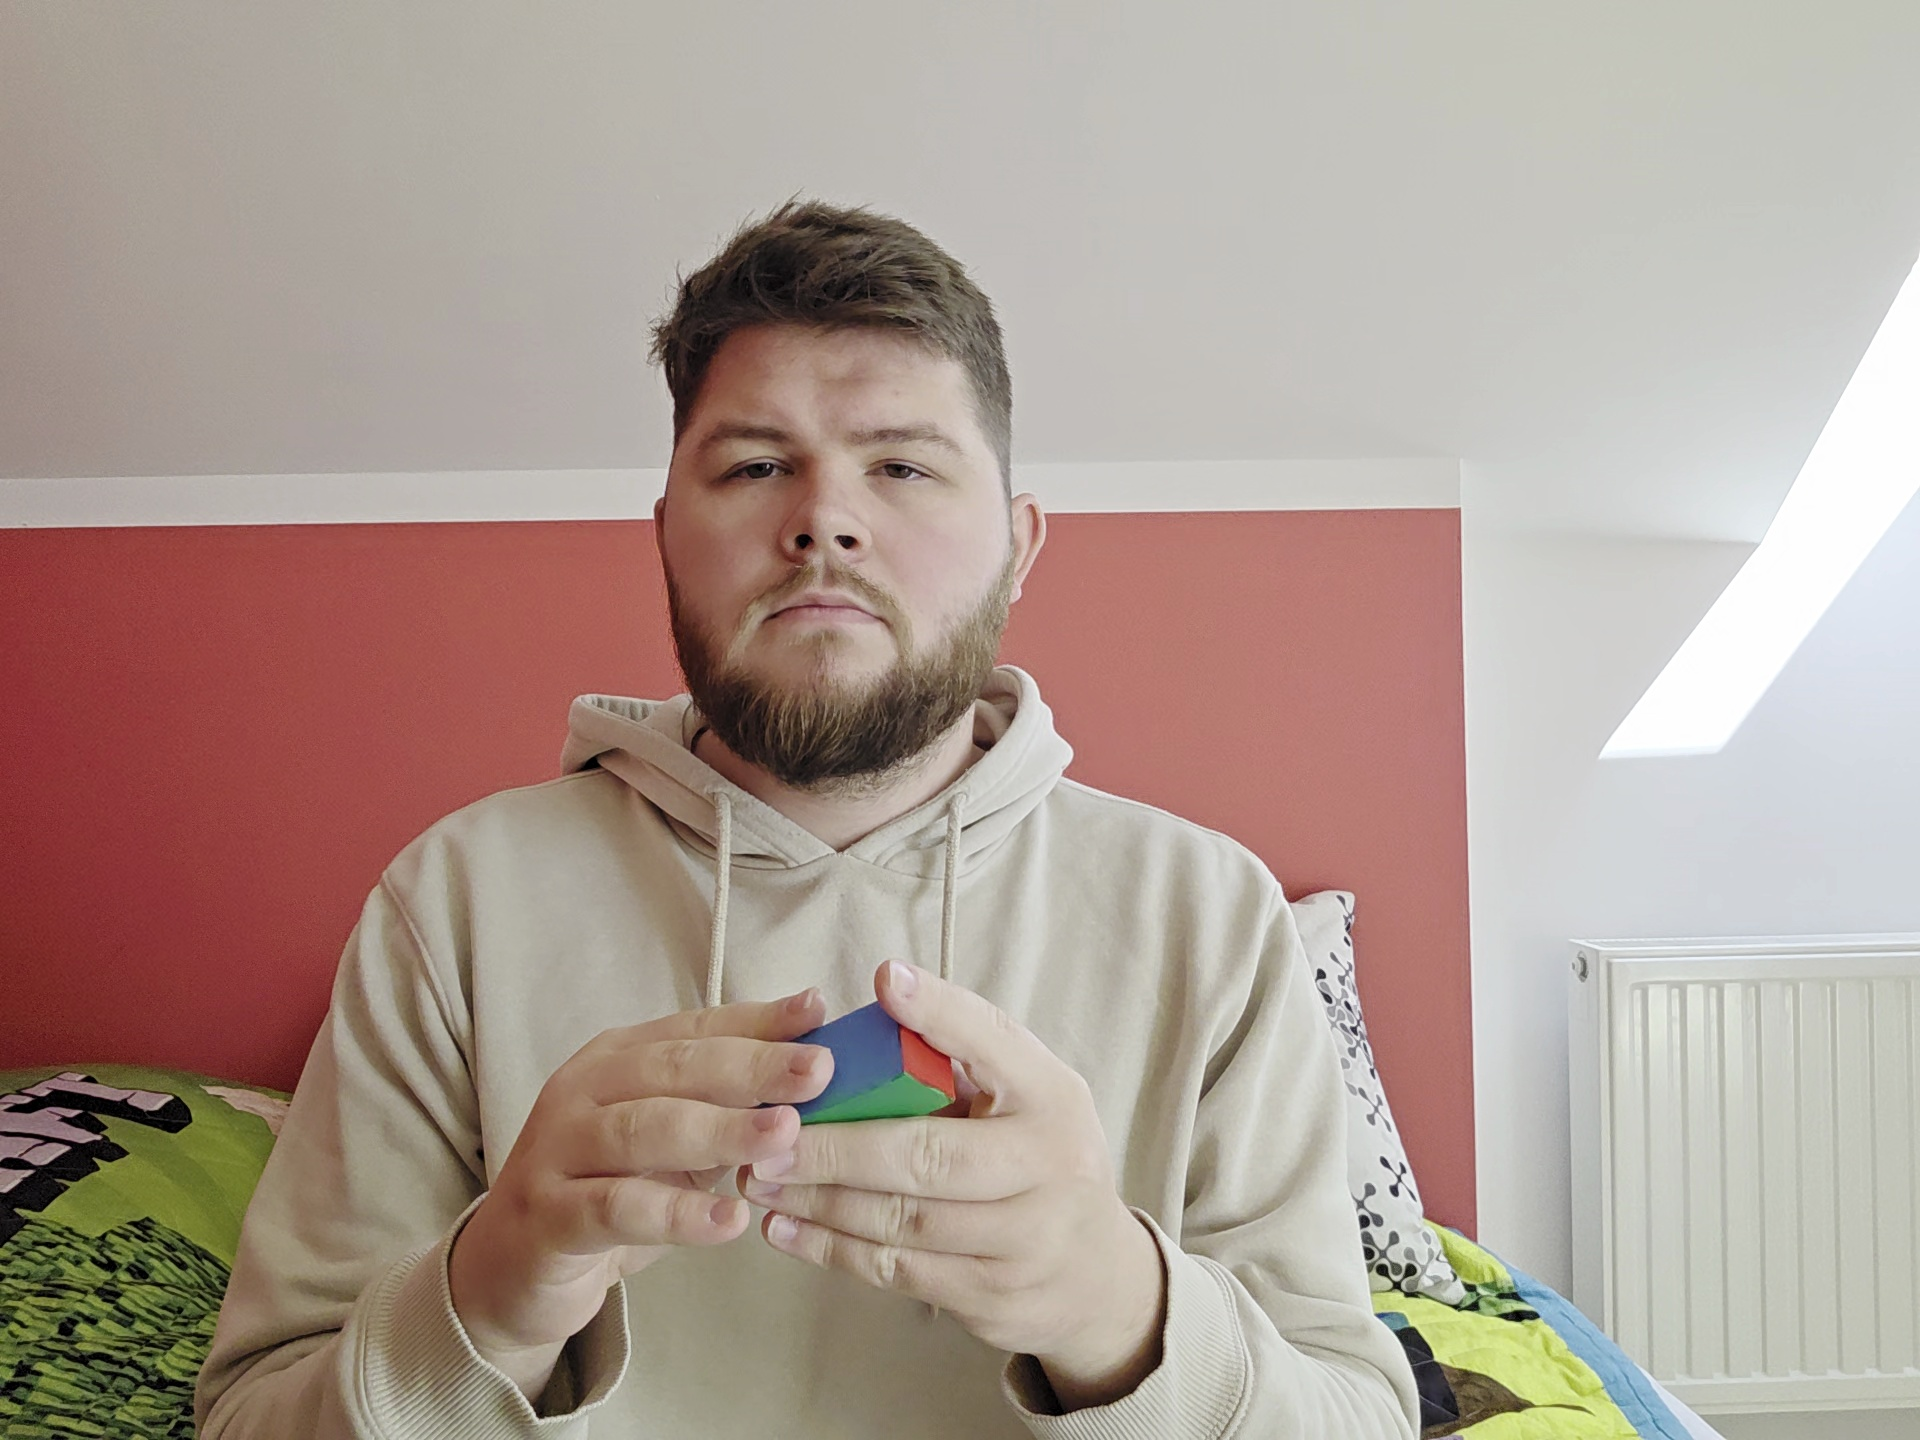
\includegraphics[width=\textwidth]{./graf/variants/frame_242_rgb.jpeg}
        \caption{Wariant kolorowy.}
        \label{fig:dataset_variants_rgb}
    \end{subfigure}
    \begin{subfigure}[b]{0.45\textwidth}
        \centering
        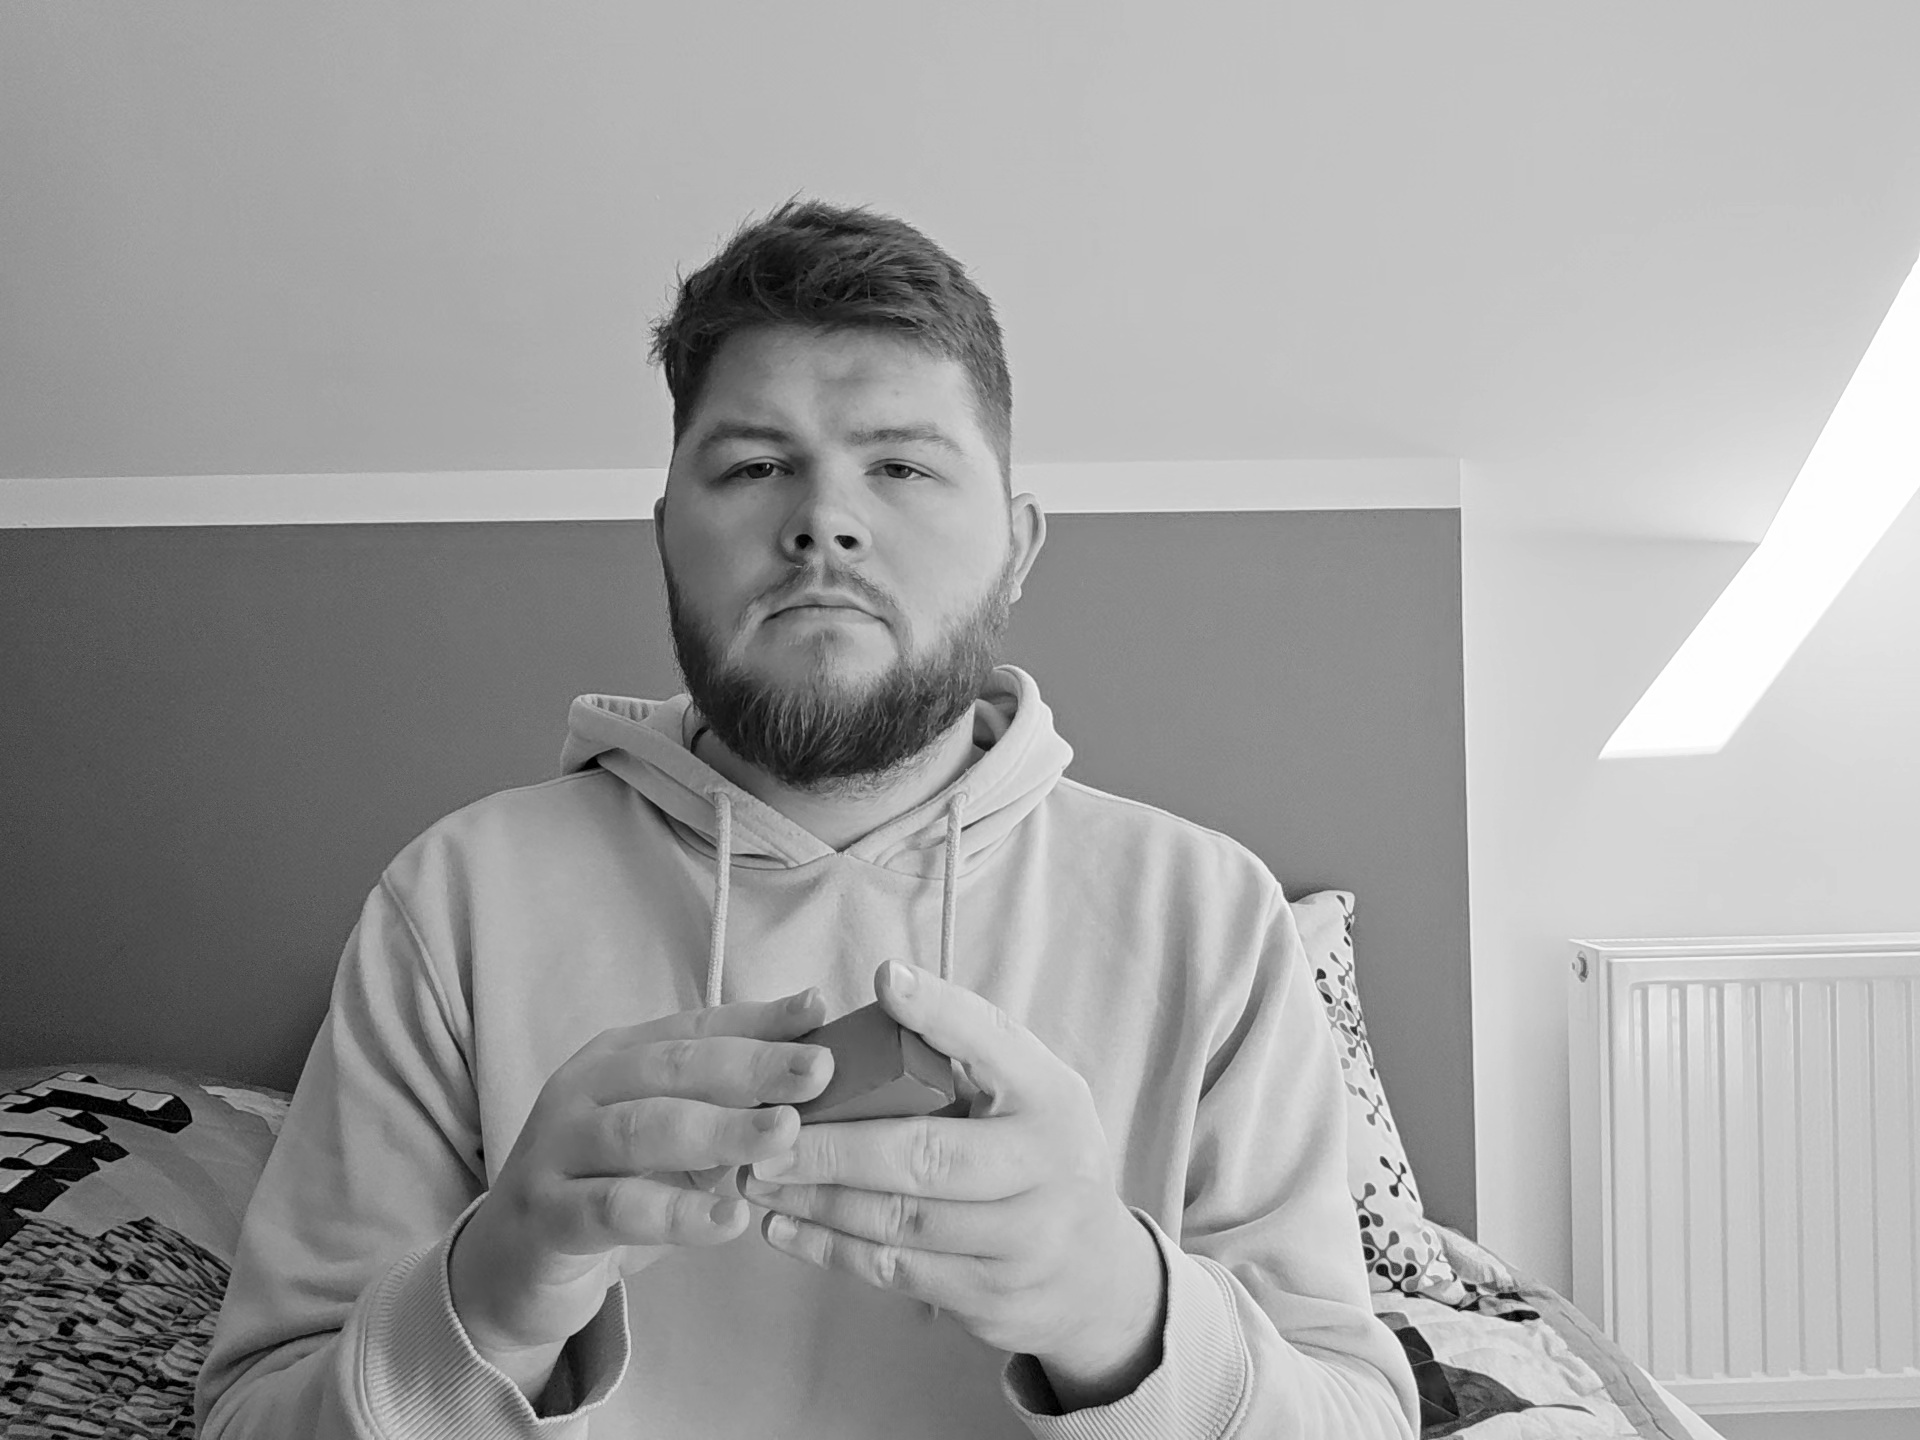
\includegraphics[width=\textwidth]{./graf/variants/frame_242_grayscale.jpeg}
        \caption{Wariant w odcieniach szarości.}
        \label{fig:dataset_variants_grayscale}
    \end{subfigure}
    \caption{Warianty danych wejściowych.}
    \label{fig:dataset_variants}
\end{figure}

\section{Metodyka eksperymentalna}

Poprawne przeprowadzenie badań wymaga ustalenia kryteriów oceny poszczególnych modeli, a także przyjęcia procedury eksperymentalnej, która umożliwi porównanie jakości detekcji pomiędzy nimi. W tym celu należy ustalić metryki oceny, a także parametry treningu modeli.

\subsection{Konfiguracja treningu modeli}

Skrypt treningowy \texttt{train.py} umożliwia konfigurację wielu parametrów treningu modelu. W eksperymentach nie wykorzystano wszystkich dostępnych opcji, a jedynie te, które uwydatnią różnice w jakości detekcji pomiędzy poszczególnymi wariantami modeli. Podczas treningu zmieniano trzy elementy konfiguracji:

\begin{itemize}
    \item \textbf{model} -- wariant modelu: YOLO26n, YOLO26s,
    \item \textbf{zbiór danych} -- warianty zbioru danych: RGB, odcienie szarości,
    \item \textbf{rozmiar obrazu} -- rozdzielczość obrazu wejściowego: $640$, $1024$.
          % \item \textbf{urządzenie} -- urządzenie, na którym przeprowadzono trening: NVIDIA A100, NVIDIA L40S, NVIDIA RTX 4060
          % \item \textbf{system operacyjny} -- system operacyjny, na którym przeprowadzono trening: Ubuntu 22.04, Windows 11.
\end{itemize}
Łącznie wytrenowano 7 modeli, które pozwoliły na przeprowadzenie eksperymentów i porównanie jakości detekcji pomiędzy nimi.

Urządzenia wykorzystane do treningu były wybierane według dostępności w danym momencie, a nie według ich wydajności. Trening na karcie graficznej NVIDIA RTX 4060 był wykonywany na lokalnym komputerze z systemem Windows~11, a treningi na pozostałych kartach odbywały się w chmurze za pomocą platformy RunPod z systemem Ubuntu~22.04. Urządzenie obliczeniowe i system operacyjny nie są zmiennymi badanymi,a ich wpływ na jakość uzyskanych modeli nie jest przedmiotem badań.

Augmentacja danych została włączona w celu zwiększenia różnorodności danych treningowych i poprawy zdolności generalizacji modeli. Wykorzystano w tym celu wbudowane w narzędzie Ultralytics YOLO mechanizmy augmentacji pozostawiając ich parametry domyślne. Obejmują one modyfikacje składowych HSV, translację, skalowanie, odbicia poziome oraz augmentację mozaikową.

Trening modeli był prowadzony do momentu braku poprawy kryterium walidacyjnego przez 50 kolejnych epok (ang. \english{early stop}). Po tym czasie trening był przerywany i uznawano, że model osiągnął swoje plateau i dalszy trening nie przyniesie znaczącej poprawy jakości detekcji. Przyjęta wartość parametru \texttt{patience} jest kompromisem pomiędzy przedwczesnym zakończeniem treningu a niepotrzebnym wydłużeniem jego czasu \cite{bib:Prechelt1998}.

Każdy trening uruchomiony został z ustawieniem ziarna generatora liczb pseudolosowych na wartość 42. Zwiększa to powtarzalność wyników oraz ułatwia odtworzenie eksperymentów w przyszłości. Wartość ta została wybrana ze względu na jej popularność w literaturze i kulturze komputerowej\footnote{Wartość 42 jest nawiązaniem do powieści Douglasa Adamsa \textit{Autostopem przez Galaktykę}, gdzie stanowi odpowiedź na  "Wielkie Pytanie o Życie, Wszechświat i całą resztę"}.

Do treningu wykorzystano następujące wersje bibliotek i narzędzi:
\begin{itemize}
    \item \textbf{Python} -- 3.11.11,
    \item \textbf{Ultralytics} -- 8.4.63,
    \item \textbf{PyTorch} -- 2.12.0,
    \item \textbf{matplotlib} -- 3.10.9,
    \item \textbf{opencv-python} -- 4.13.0.92,
    \item \textbf{CUDA} -- 13.2.
\end{itemize}

\subsection{Metryki oceny}

Do oceny poszczególnych modeli wykorzystano metryki zwracane przez bibliotekę Ultralytics: precision, recall, $mAP50$, $mAP50\text{-}95$ oraz macierze pomyłek. Dodatkowo obliczano wartość $F1$-score dla najlepszego modelu w każdym eksperymencie. Szczegółowe opisy każdej z użytych metryk znajdują się w sekcji~\ref{s:metryki}.

Dokładne przebiegi każdego treningu znajdują się w pliku \texttt{results.csv}, a porównanie najlepszej epoki treningu z ostatnią przedstawia plik \texttt{run\_stats.json}.

Najważniejszą z używanych metryk jest $mAP50\text{-}95$, ponieważ uwzględnia ona jakość detekcji dla wielu progów IoU i pozwala na ocenę zarówno jakości lokalizacji, jak i klasyfikacji obiektów \cite{bib:ultralytics_yolo_metrics}. Jako metryka pomocnicza użyto siostrzaną metrykę $mAP50$, która jest łatwiejsza do interpretacji i ukazuje skuteczność detekcji przy mniej rygorystycznych kryteriach. Kolejno, metryki precision i recall umożliwiają ocenę jakości detekcji w kontekście liczby wykrytych obiektów, a ich średnia harmoniczna $F1$-score opisuje kompromis pomiędzy nimi. Niezwykle przydatne okazują się również macierze pomyłek, na których podstawie można określić, które klasy są najtrudniejsze do wykrycia i które są najczęściej mylone z innymi.

Do porównania należy wykorzystać metryki, które zostały wyznaczone na zbiorze testowym, a nie na zbiorze walidacyjnym. Zbiór walidacyjny służy wyłącznie do oceny jakości predykcji podczas treningu do wyznaczenia najlepszej epoki treningu, podczas gdy zbiór testowy jest wykorzystywany do końcowej oceny modelu. Ważne jest również, aby przy każdym eksperymencie używać dokładnie tego samego zbioru testowego, aby zachować miarodajne porównanie poszczególnych modeli. Wyniki tej oceny stanowią podstawę do porównania modeli przedstawionego w rozdziale~\ref{c:badania}.

Oprócz metryk jakości detekcji przy końcowym porównaniu modeli uwzględniono liczbę ich parametrów, koszt obliczeniowy wyrażony w GFLOPs, rozmiar pliku modelu oraz czas inferencji i wynikającą z niego liczbę przetwarzanych klatek na sekundę. Wartości te zebrano w dwóch niezależnych seriach pomiarowych na pojedynczym urządzeniu.

Nie porównywano pełnego czasu odpowiedzi ponieważ jest on silnie zależny od używanego urządzenia obliczeniowego, przepustowości sieci oraz obciążenia systemu operacyjnego. Każdy przypadek wdrożenia systemu należy oceniać indywidualnie, na podstawie wyników eksperymentów przeprowadzonych na docelowym sprzęcie i w docelowych warunkach pracy.

\subsection{Procedura eksperymentalna}
\label{ssec:procedure}

Aby móc dokonać porównania jakości detekcji pomiędzy poszczególnymi wariantami modeli należy podzielić je na eksperymenty. Każdy z nich polegał na wytrenowaniu kilku, porównywalnych modeli, które różniły się pojedynczym parametrem. Wykonano następujące eksperymenty:

\begin{enumerate}[label=\textbf{Eksperyment \Alph*:}, leftmargin=*, align=left]
    \item Porównanie jakości detekcji pomiędzy rozmiarami modelu YOLO26 \texttt{n} i \texttt{s} dla danych wejściowych w wariancie kolorowym. Pozwoli to ocenić wpływ skali modelu i ilość jego parametrów na jakość detekcji.
    \item Porównanie jakości detekcji pomiędzy wariantami z różnymi rozdzielczościami obrazu wejściowego: $640$ oraz $1024$. Pozwoli on ocenic wpływ rozdzielczości obrazu na jakość detekcji.
    \item Porównanie jakości detekcji pomiędzy wariantami danych: kolorowym i w odcieniach szarości. Pozwoli to ocenić, czy usunięcie informacji o barwie wpływa na jakość detekcji i czy model jest w stanie skutecznie rozpoznać obiekty bez wykorzystania informacji o kolorze.
\end{enumerate}

Przedstawione eksperymenty pozwalają ocenić, czy możliwe jest skuteczne rozpoznawanie trzymanych obiektów trójwymiarowych bez informacji o kolorze, a także czy możliwe jest uzyskanie zadowalających wyników przy użyciu modeli o mniejszej liczbie parametrów. Wyniki poszczególnych eksperymentów zostały przedstawione w rozdziale~\ref{c:badania}.